\graphicspath{{figures/chapter3/}}
\onehalfspacing

\chapter{UAV photogrammetry for annual glacier reconstruction (2015-2023)}\label{ch:3}

\vfill

\newthought{This chapter is based on:}

\noindent Ioli, F., Bianchi, A., Cina, A., De Michele, C., Maschio, P., Passoni, D., \&
Pinto, L. (2021). Mid-Term Monitoring of Glacier’s Variations with UAVs: The Example of
the Belvedere Glacier. Remote Sensing, 14(1), 28.
\url{https://doi.org/10.3390/rs14010028}

\newpage

\section{Introduction\textcolor{red}{TODO}}\label{sec:3:intro}

This chapter presents the extensive and continuous monitoring activity that has been carried out since 2015
and aimed at investigating the annual evolution of the Belvedere Glacier with UAVs-based photogrammetry and in-situ GNSS measurements.
The monitoring activity was designed and conducted jointly by the Department of Civil and Environmental Engineering (DICA) 
of Politecnico di Milano and the Department of Environment, Land and Infrastructure Engineering (DIATI) of Politecnico di Torino. 
Moreover, the DREAM projects (DRone tEchnnology for wAter resources and hydrologic hazard Monitoring), 
involving teachers and students from Alta Scuola Politecnica (ASP) of Politecnico di Torino and Milano, 
contributed to the campaign from 2015 to 2017.

Every year, fixed-wing UAVs and quadcopters were used to remotely sense the glacier and build 
high-resolution 3D photogrammetric models, which are employed for investigating the glacier kinematics.
The series of point clouds is then used to estimate the ice volume variations of the glacier, while the orthophotos
are used to estimate the ice flow velocity and glacier retreat. 


\textcolor{red}{The goal of this work is ...}

\textcolor{red}{add short intro on open data ...}


\section{Instruments and datasets}\label{sec:3:instrument}

Every year, the monitoring activity involved the acquisition of punctual GNSS measurements 
and UAV images spread all over the glacier. 
This section introduces the data acquired in this study from 2015 to 2023.

\subsection{GNSS measurements}\label{sec:3:gnss}

Yearly GNSS measurements of permanent targets deployed across the glacier were conducted. 
These targets served a dual purpose: as GCPs/CPs for photogrammetric block processing and as high-accuracy 
reference points for evaluating glacier kinematics derived from photogrammetry. 
The targets were materialized using square cross patterns printed on polypropylene sheets and anchored to 
large rocks and boulders (\figref{fig:3:belvedereGCP}b).
Approximately 25 targets were deployed on the glacier itself (designated as as \textit{moving targets} or 
\textit{M\#} in \figref{fig:3:belvedereGCP}a), while 24 targets were placed on stable areas along the moraines 
(labelled as \textit{stable targets} or \textit{S\#} in \figref{fig:3:belvedereGCP}a). 

Every year, the condition of each target was checked and, if one was damaged or
destroyed, the polypropylene sheet was replaced by keeping the same location of the
center (i.e., by using the same fisher plugs). 
During the years, some targets were lost, and therefore new ones were materialized, close 
to the location of the lost ones (e.g., M29bis).

All targets were surveyed with dual frequency geodetic quality GNSS receivers: 
Leica GPS VivaGS14 and Leica GPS1200+.
The measurements were framed within the official Italian reference system ETRF2000
at the epoch 2008.0, projected in UTM 32N (RDN2008 / UTM zone 32N, EPSG:7791).

The measurement techniques employed in the survey have evolved over time.
Before 2021, target positions on the lower glacier (where GSM network coverage was available) 
were determined using nRTK relative to CORS permanent stations (either HxGN SmartNet or SPIN GNSS).
These points were occupied for at least two 5-second intervals. 
In contrast, upper glacier targets were surveyed using static sessions of approximately 10 
minutes, with raw data post-processed relative to local master stations located in stable areas 
(S12 or S20, see \figref{fig:3:belvedereGCP}a).

Since 2021, GNSS measurements were conducted in RTK mode using a local base station 
(\textit{S12} or \textit{S20}).
The real-time corrections were streamed from the base to the rover by a radio link connection. 
his approach has significantly reduced measurement time in the upper glacier, requiring seconds 
rather than minutes per occupation, as was for static processing.
Additionally, the local-base RTK method improves internal coherence among measurements, 
as well as tropospheric and ionospheric error modeling due to shorter baselines compared to 
the nRTK approach.

The accuracy of GNSS measurements was evaluated empirically by comparing repeated
measurements over stable targets carried out in different years.
RMSE of \qty{1.5}{\centi\meter} in planimetry and \qty{3}{\centi\meter} in elevation were
obtained.


\begin{figure}
    \centering
    \subcaptionbox{\label{fig:3:3:studyarea:map}}{
        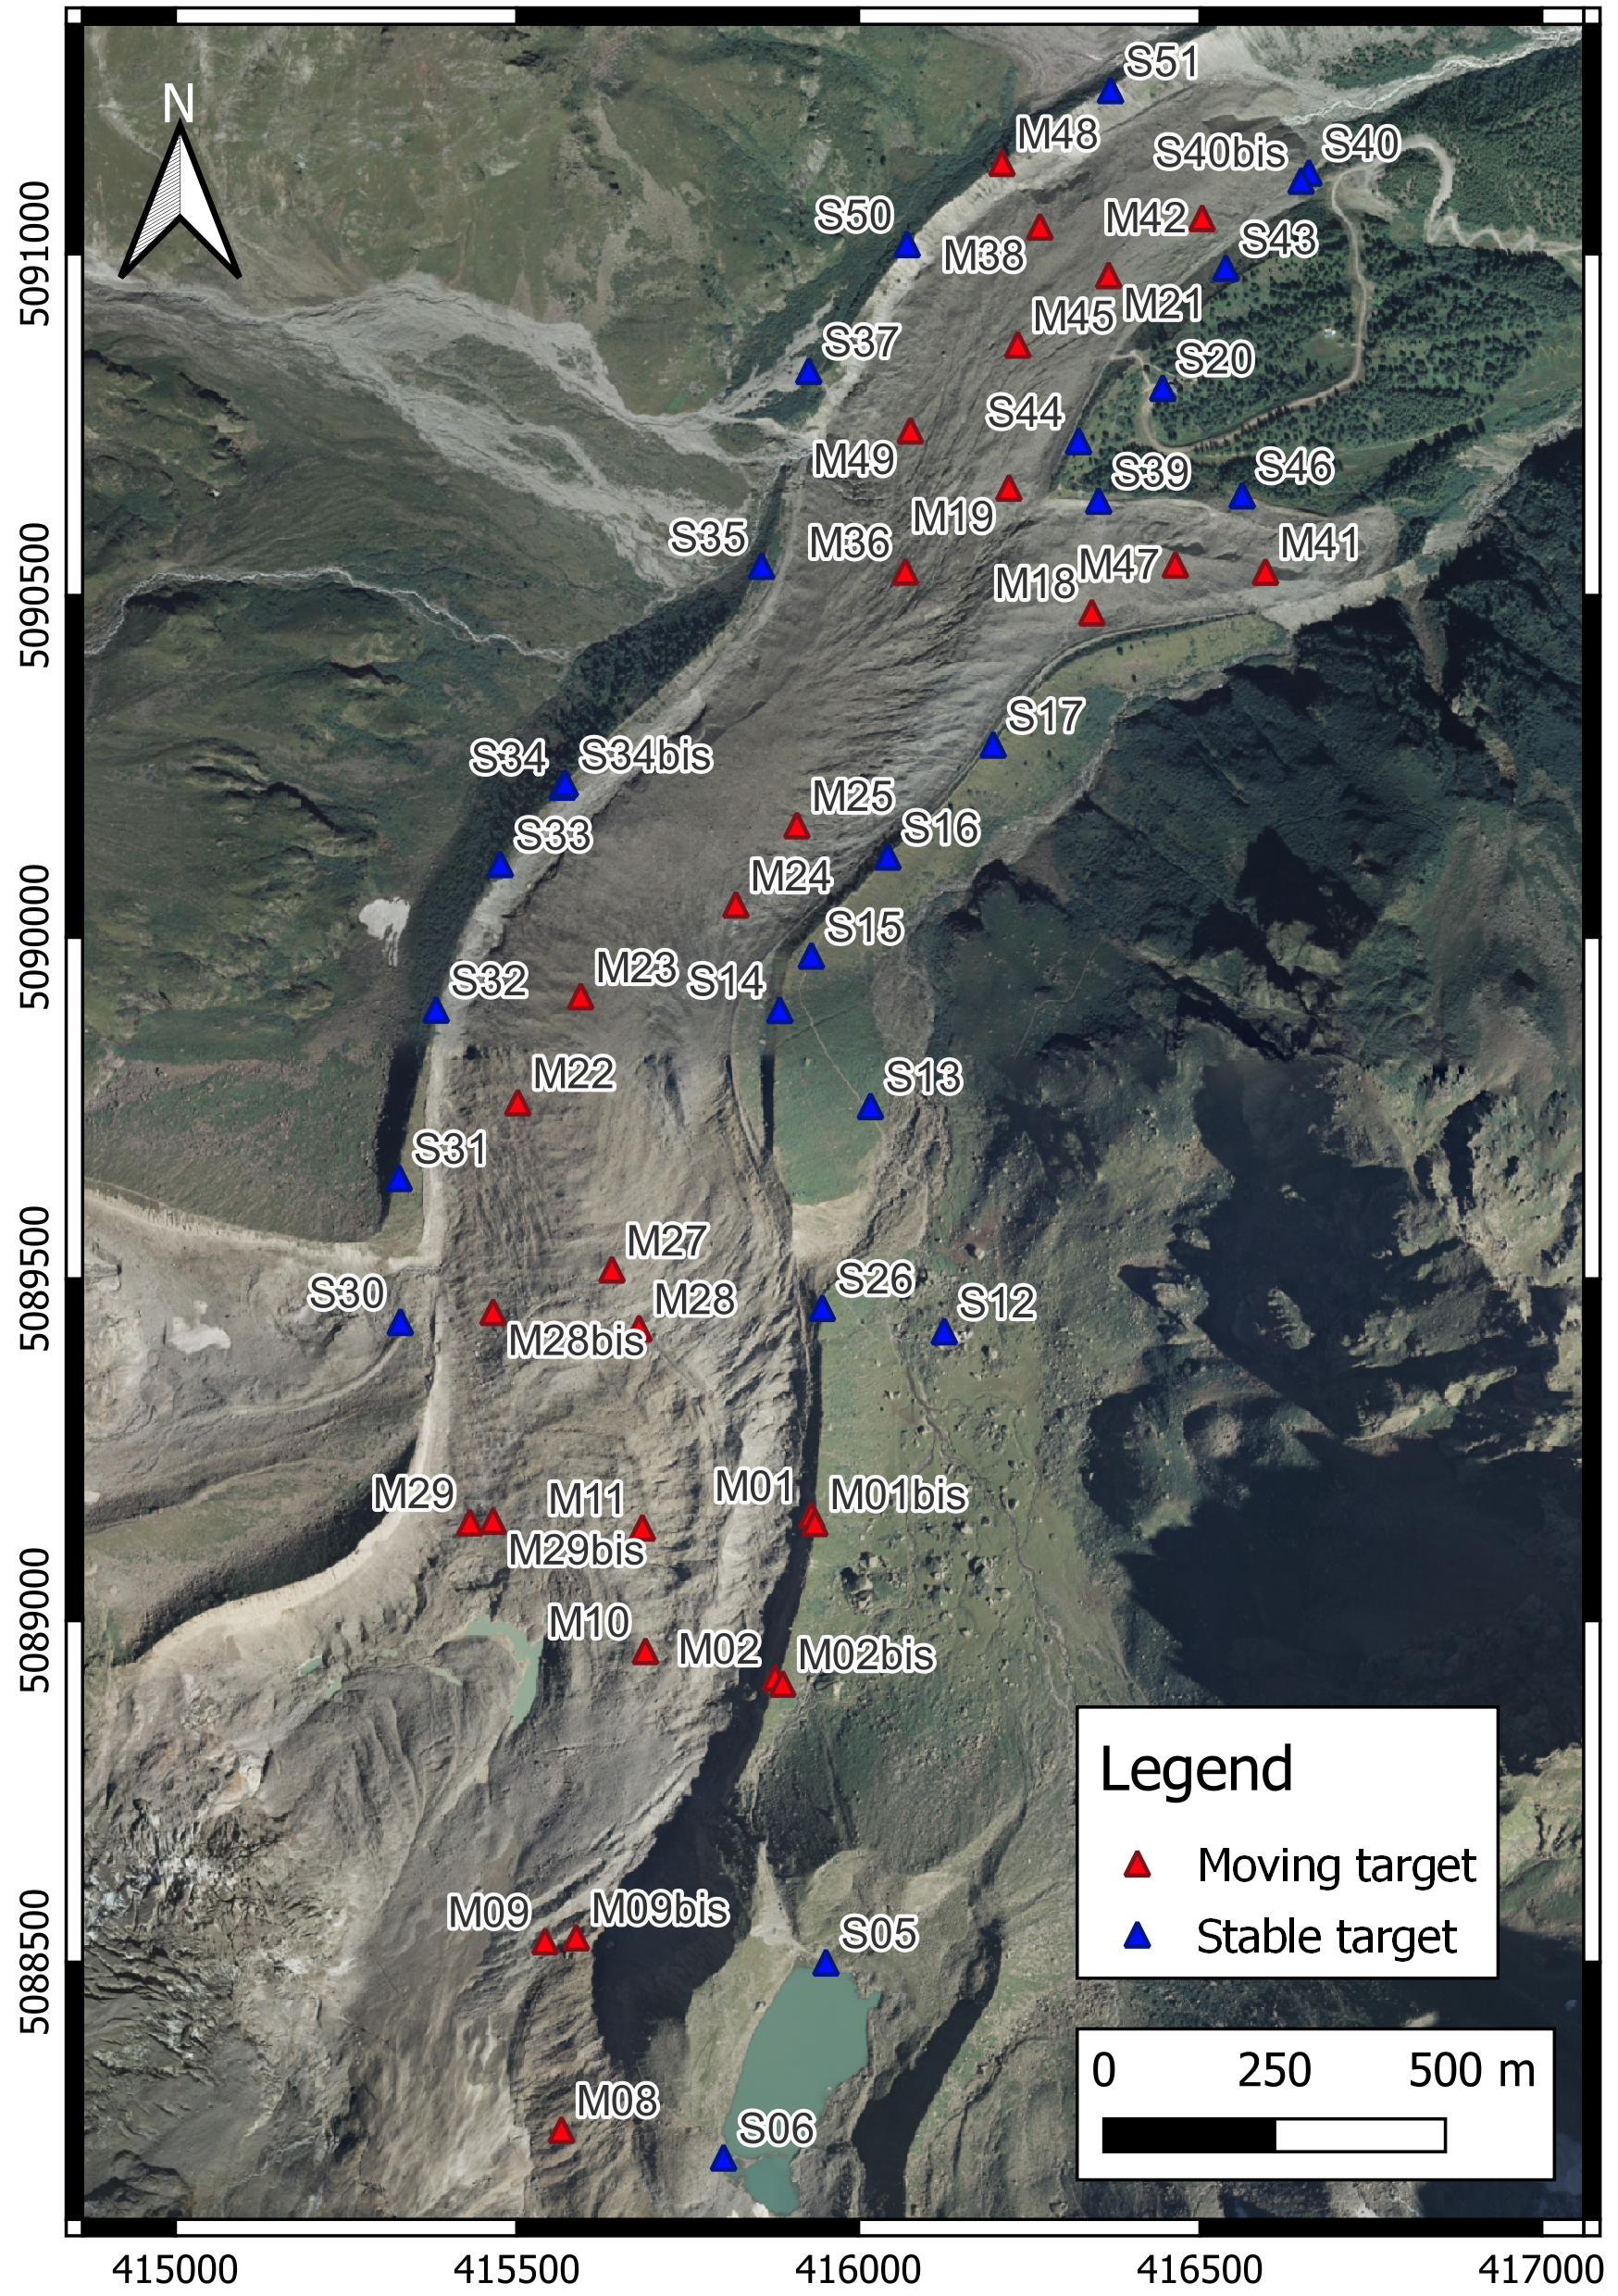
\includegraphics[width=.6\textwidth]{belvedereGCP.png}
    }
    \subcaptionbox{\label{fig:3:3:studyarea:pic}}{
        \includegraphics[width=.35\textwidth]{target.jpg}
    }
    \caption{(\textbf{a}) An example of a photogrammetric target deployed over the
        glacier moraine; (\textbf{b}) location of the targets used for the
        photogrammetric
        surveys. For~each year, a~subset of the targets were used as GCPs, while the
        remaining
        as~CPs.}
    \label{fig:3:belvedereGCP}
\end{figure}


\subsection{UAV flights}\label{sec:3:uav-flights}

The long duration of the monitoring campaign, challenging environment, and involvement of 
multiple research groups led to the use of various UAV platforms and cameras over time. 
\tabref{tab:3:datasets} provides a detailed summary of the equipment (UAV and camera) employed, while 
\tabref{tab:3:camere} lists the main sensor and lens specifications for each camera.

In 2015 and 2016, a ready-to-fly fixed-wing SenseFly eBee equipped with a compact camera Canon
PowerShot S110 was used for whole glacier surveys.
Due to technical problems, the year 2017 saw the use of different UAVs (both fixed-wing and quadcopters)
and camera combinations (\tabref{tab:3:datasets}). 
From 2018 to 2020, a low-cost recreational Parrot Disco FPV fixed-wing UAV (wingspan 1.15 m, weight 750 g) 
was adapted to carry a lightweight Hawkeye Firefly 8S action camera.

In 2021, a professional-grade DJI Matrice 210 V2 quadcopter was employed, carrying a 
DJI ZenMuse X5s camera featuring a Micro 4/3 sensor and a 15 mm lens. 
Since 2022, the UAV platform has been upgraded to a DJI Matrice 300 RTK quadcopter
paired with a full-frame DJI Zenmuse P1 camera and a DL 35 mm F2.8 LS ASPH lens.
While this setup offered superior image quality, the longer focal length necessitates 
higher flight altitudes to maintain a consistent GSD with the previous surveys.
Furthermore, the DJI Matrice 300 RTK was equipped with an RTK GNSS receiver, enabling 
decimeter-level accuracy in recording the camera position for each shot. 
This precision was achieved through a local GNSS base station positioned near the take-off 
location, which streamed real-time corrections to the drone via DJI's proprietary link.

UAV flights were conducted automatically by using ground station software packages
developed by UAV manufacturers and UgCS\footnote{\url{https://www.sphengineering.com/flight-planning/ugcs}}
flight planning software.
The flights were designed to have GSD ranging between \qtylist{5;10}{\centi\meter}, and
to guarantee \qty{\sim 80}{\percent} of longitudinal and \qty{\sim 60}{\percent} of
transversal overlap.
Average image GSD values and number of GCPs and CPs, used respectively to orient the
images and to assess the quality of the photogrammetric blocks, are summarized in
\tabref{tab:3:datasets}.

\begin{table}[p]
    \small
    \centering
    \caption{Summary of the characteristics of the surveys.}
    \begin{tabular}{c  m{1.8cm} m{3.5cm} m{4.2cm} c c c }
        \toprule
        Year                                                              & Date
                                                                          & UAV
                                                                          & Camera
                                                                          & GSD
                                                                          & GCP
                                                                          & CP
        \\
                                                                          &
                                                                          &
                                                                          &
                                                                          & [m/px]
                                                                          & [\#]
                                                                          & [\#]
        \\
        \midrule
        2015                                                              & A.
        8.10\newline B. 23.10                                             &
        SenseFly eBee                                                     & Canon
        PowerShot S110                                                    & 0.07
                                                                          & 24
                                                                          & 11
        \\[4mm]
        2016                                                              & 20.10
                                                                          & SenseFly eBee
                                                                          & Canon
        PowerShot S110                                                    & 0.09
                                                                          & 31
                                                                          &
        15
        \\[4mm]
        2017                                                              & A.
        5.10\newline B. 15.11\newline C. 16.11                            & A. SenseFly
        eBee \newline B. SenseFly eBee Plus\newline  C. DJI Phantom 4 Pro & A. Canon
        PowerShot
        S110  \newline B. SenseFly S.O.D.A \newline C. DJI FC6310         & 0.06
                                                                          & 27
                                                                          & 8
        \\[4mm]
        2018                                                              & 23-25.07
                                                                          & Parrot Disco
                                                                          & Hawkeye
        Firefly 8S                                                        & 0.05
                                                                          & 27
                                                                          &
        13
        \\[4mm]
        2019                                                              & 29.07-2.08
                                                                          & Parrot Disco
                                                                          & Hawkeye
        Firefly 8S                                                        & 0.06
                                                                          & 26
                                                                          &
        10
        \\[4mm]
        2020                                                              & A. 26-27.07
        \newline B. 9.08                                                  & A.
        Parrot Disco\newline B. DJI Phantom 4 Pro                         & A. Hawkeye
        Firefly 8S\newline B. DJI FC6310                                  &
        0.05                                                              & 29
                                                                          & 12
        \\[4mm]
        2021                                                              & 29.07-2.08
                                                                          & DJI Matrice 210 V2
                                                                          & DJI ZenMuse x5s
                                                                          & 0.04
                                                                          & 23
                                                                          &
        9
        \\[4mm]        
        2022                                                              & 28.07-29.07
                                                                          & DJI Matrice 300 RTK
                                                                          & DJI Zenmuse P1 - 35 mm
                                                                          & 0.03
                                                                          & 22
                                                                          &
        19
        \\[4mm]
        2023                                                              & 25.07-27.07
                                                                          & DJI Matrice 300 RTK
                                                                          & DJI Zenmuse P1 - 35 mm
                                                                          & 0.03
                                                                          & 23
                                                                          &
        9
        \\[4mm]        
        \bottomrule

    \end{tabular}
    \label{tab:3:datasets}
\end{table}

\begin{table}[p]
    \centering
    \small
    \caption{Summary of the characteristics of the cameras employed.}
    \begin{tabular}{c c c c c c}
        \toprule
        Camera                        & Sensor                        & Sensor Size
                                      & Focal length                  & Image size
                                      & Pixel size
        \\
                                      &                               &
        [\SI{}{\milli\meter\squared}] & \newline[\SI{}{\milli\meter}] & [\SI{}{\pixel}]
                                      & \newline[\SI{}{\micro\meter}]
        \\

        \midrule
        Canon PowerShot S110          & 1/1.7" CMOS                   & $7.44\times5.58$
                                      & 5.2                           & $ 4000 \times
            3000
        $                             & 1.9
        \\
        SenseFly S.O.D.A              & 1" CCD                        & $13.2\times8.8$
                                      & 10.6                          & $5472 \times
        3648$                         & 2.4
        \\
        DJI FC6310                    & 1" CMOS                       & $13.2\times8.8$
                                      & 8.8                           & $5472 \times3648$
                                      & 2.4
        \\
        Hawkeye Firefly 8S            & 1/2.3" CMOS                   & $6.17\times4.56$
                                      & 3.8                           & $5472 \times3648$
                                      &
        1.34
        \\
        DJI ZenMuse x5s               & 4/3" CMOS                     & $17.3\times13$
                                      & 15                            & $5280 \times
        3956$                         & 3.3 
        \\
        DJI Zenmuse P1 - 35 mm        & FullFrame CMOS                & $35.9\times24$
                                      & 35                            & $8192 \times
        5460$                         & 4.4
        \\
        \bottomrule
    \end{tabular}
    \label{tab:3:camere}
\end{table}

\subsection{Challenges and adaptations in the 2017, 2018 and 2020 surveys}\label{sec:3:problems} 

Conducting annual monitoring campaigns in alpine environments poses logistical and environmental
challenges, including limited accessibility in certain areas and unpredictable weather. 
These factors directly impacted the 2017 and 2020 surveys.

Adverse weather and logistical constraints necessitated splitting the 2017 survey across 
multiple dates, requiring using different UAVs and cameras (see \tabref{tab:3:datasets}). 
Consequently, the photogrammetric model was built in three parts. 
The central portion corresponds to a survey carried out in October, while the snow-covered 
upper and lower sections were acquired in November (\figref{fig:3:ortophoto}c).

Technical issues arose during the 2020 survey when an elevon servo failed during landing and
caused the fixed-wing UAV to crash.
To complete the survey, a DJI Phantom 4 Pro quadcopter was employed 14 days later to survey 
the upper part of the glacier (see the different colors in the orthophoto of
\figref{fig:3:ortophoto}f).
However, the harsh terrain and the presence of crevasses in the upper part of the glacier 
prevented the measurement of additional GCPs to constrain the model in this region. 
This necessitated co-registering the Phantom 4 Pro model with the 2019 data, 
using stable rock features along the moraines as reference points. 
This approach was less accurate than measuring GCPs directly on the field and yielded an
RMSE on CPs of \SI{0.36}{\meter} (see \figref{fig:3:CP_errors}), \SI{\sim 7}{}~times the GSD.
Nevertheless, the area affected by this problem consisted of the upper accumulation area only
and it was rather limited compared to the whole Belvedere~Glacier.

The project timeline also led to a shift in survey periods from autumn (2015-2017) 
to summer (2018-2023).
This change means that the timespan between the October/November 2017 and July 2018 
surveys does not encompass the summer (neither August 2017 nor August 2018 was included), 
which is the period of maximum glacier ablation and surface velocity. 
Consequently, volume variation and ice flow velocity estimated between 2017 and 2018 reflect
primarily winter conditions and are not directly comparable to other years, as they underestimate
the actual annual average statistics.

\section{Metodology}\label{sec:3:methodology}

\subsection{SfM workflow}\label{sec:3:sfm}

To generate photogrammetric models of the glacier, UAV imagery was processed using 
Agisoft Metashape 1.8.5\footnote{\url{https://www.agisoft.com}}.
Each year, a minimum of 22 GCPs distributed across the glacier were used for image 
orientation, while at least 8 CPs served for model quality assessment.  
All GCPs and CPs were manually collimated within the images.

Tie Points (TPs) were detected and matched by Metashape on full-resolution images (which
corresponds to \textit{high accuracy} parameter in Metashape).
Image External Orientation (EO) and TPs world coordinates were estimated by solving the
Bundle Block Adjustment (BBA).
TPs with the worst reprojection error on images, which likely originated from false
matches, were removed and the BBA was solved again to improve the quality of the BBA solution.
This process was iterated more times until the TP mean reprojection error had dropped below
\SI{\sim 0.8}{\pixel}.
Camera internal orientation was estimated by self-calibration
\citep{Fraser2013, Cramer2017}, because of its instability in the cameras employed.

Agisoft Metashape computed dense 3D reconstruction with proprietary MVS
algorithms~\citep{Dallasta}.
Depth maps and dense point clouds were obtained from images downsampled by a factor of 4,
in~order to reduce the computational time (\textit{medium quality} parameter of the dense
cloud generation in Metashape).
Triangulated mesh surfaces and photorealistic textures were computed.

DSMs with a resolution of \SI{0.5}{\meter\per\pixel} were derived from the mesh model.
Finally, orthophotos with a GSD of \SI{0.10}{\meter\per\pixel} were obtained by
projecting the most nadiral images over the mesh model (\figref{fig:3:ortophoto}).

\subsection{Glacier flow velocity}\label{sec:3:method_velocity}

In debris-covered glaciers, surface debris and boulders primarily move in conjunction with the underlying
ice flow, making them valuable proxies for evaluating glacier kinematics through tracking 
techniques~\citep{Dehecq2015, Sam2016, Blothe2021}.

In-situ GNSS measurements of the \textit{moving targets} anchored to large rocks (see~\secref{sec:3:gnss})
was used as a method for deriving glacier surface flow velocities.
These punctual measurements, labeled as \textit{GNSS}, provided high-accuracy, 
estimated at approximately \qty{\sim 3}{\centi\meter} (see Section~\ref{sec:3:gnss}).
Assuming measurements of the same target at two consecutive years as independent, the expected standard deviation 
of the velocity was computed by propagating the variance as \qty{\pm 0.04}{\meter\per\year}.
Therefore, GNSS measurements were considered the most reliable reference for flow velocity estimation.
However, due to the limited number of GNSS measurement points across the glacier, they are insufficient 
for deriving a complete glacier velocity field.

A powerful approach for deriving glacier flow velocity using remote sensing involves DIC or 
feature tracking algorithms~\citep{ahn_box_2010, Giordan2016, Hadhri2019}.
At its core, DIC tracks distinct pixel patterns across a time series of images, employing cross-correlation to quantify 
surface displacements. 
This implies iteratively analyzing subsets of the reference image (often referred to as \textit{templates} 
or \textit{windows}), pinpointing the location of maximum similarity within a search area in the subsequent 
image by cross-correlation in spatial \citep{Scambos1992} or frequency domain \citep{rolstad1997}.
This shift represents the displacement of the tracked feature.
Initially applied to glaciers by \cite{Scambos1992}, DIC is now widely used to analyze optical satellite imagery
\citep{Scambos1992, Scherler2008, Heid2012_evaluation_xcorr} or high-resolution orthophotos derived by aerial or 
UAV photogrammetry \citep{immerzeel2014, Chudley2019, ioli2021mid}. \textcolor{red}{(This is more an intro... think about moving...)}

The presence of snow and significant environmental variations between orthophotos from 2015 to 2018 (\figref{fig:3:ortophoto}),
prevented the use of automated image matching algorithms. 
Consequently, we relied on the visual identification of characteristic features (e.g., sharp edges of large rocks) across multiple 
orthophotos \citep{Lucchitta1986} for tracking surface elements and deriving velocity fields. 
We refer to these points as \textit{MAN}.

Assuming collimation standard deviation of \SI{\sim 2}{\pixel} and considering the planimetric accuracy of 
the orthophotos of \SI{\sim 0.1}{\meter} (Figure~\ref{fig:CP_errors}), 
the~standard deviation of the velocity obtained from MAN points was estimated as \SI{\pm 0.3}{m/y} 
by variance propagation (covariances were neglected, assuming the orthophotos as independent).  

While less precise than DIC, manual selection by a human operator ensured high matching reliability. 
To maintain uniform distribution, features were selected on a \qtyproduct{100 x 100}{\metre} grid whenever possible, resulting 
in approximately 130 points (with approximately (approximately one point every \qty{10000}{\meter\squared})).  
Unfortunately, some points were lost over time, leaving only 115 identifiable on the 2020 orthophoto.

From 2018 onwards, consistent acquisition periods (end of July) and snow-free conditions enabled the use of 
DIC for comprehensive velocity field derivation. 
We employed the open-source Local Adaptive Multiscale Image Matching Algorithm (LAMMA)~\citep{Dematteis2022}, 
LAMMA adopts a hierarchy structure of patch grids of increasing spatial resolution and
uses locally-adaptive search area sizes, according to the displacements already
obtained in the neighboring region.
Lamma was originally written in Matlab\footnote{\url{https://github.com/niccolodematteis/LAMMA}}, but we have 
recently translated it into Python for multitemporal processing of stereo images \citep{ioli2024deep} and 
published it as an open-source library, named pyLamma\footnote{\url{https://github.com/franioli/pylamma/}}.

As a correlation function, we used the cosine similarity applied to orientation images \citep{Dematteis2021}, 
which is less sensitive to chromatic variation changes (e.g., due to to shadows or snow patterns) and is known 
to perform well in glacier environments \citep{Heid2012_evaluation_xcorr, Dematteis2019}.
The cosine similarity function is defined as \citep{Dematteis2022}:
\begin{equation}
\text{CXC}(r,c) = \frac{1}{RC} \sum_{r,c} \mathrm{Re} \left( A_{\text{or}}^{*}(i,j) \cdot B_{\text{or}}(i+r,j+c) \right)
\end{equation}
where $A_{or}$ and $B_{or}$ denotes the complex conjugate and are the orientation images of the 
reference and slave patches, respectively. 
An orientation image is defined as $ I_{\text{or}} = \frac{I_x}{|I_x|} + i\frac{I_y}{|I_y|} $, 
where are the first derivatives of the image intensity in the two dimensions \citep{fitch2002_OC}.

To achieve subpixel displacement sensitivity, LAMMA considers the sub-region of the similarity function centred 
in its maximum value and it oversamples this sub-region using bicubic interpolation \citep{Dematteis2022}.
Then, the subpixel displacement is the peak's position of the oversampled correlation function \citep{Debella_Gilo2011}.
 
The noise level of DIC was evaluated by applying it to stable areas. \textcolor{red}{CONTINUE...}

\subsection{Volume variations}\label{sec:3:method_volumes}

To compute glacier volume variation $ \Delta V $, consecutive DSMs were differentiated
by employing a DEM of Difference (DOD) approach.
To this end, the tool \textit{Compute 2.5D volume} implemented in 
CloudCompare~\footnote{Cloudcompare: \url{https://www.danielgm.net/cc/}} was used.
First, photogrammetric dense clouds were gridded by projecting points along the vertical
direction onto a planar surface, resulting in DSMs with a \qtyproduct{0.5x0.5}{\meter} ground resolution.
This resolution balances robust height estimation (by averaging a sufficient number of points per cell) 
with the ability to resolve finer-scale glacier morphology.
A manually created mask delineated the glacier surface within each DSM, ensuring only 
relevant areas were analyzed.  
DSMs from consecutive years were then subtracted pixel-by-pixel, yielding the height 
difference for each raster cell.

A simplified approach was initially used to estimate volume variation variance, 
treating each DSM as a mono-dimensional random variable with variance equal to the squared 
vertical RMSE computed on CPs.  
While providing a preliminary idea, a more rigorous uncertainty estimation would require 
several additional considerations.
Firstly, to propagate variance accurately, we need the full covariance matrix of each DSM. 
This information is not provided by the SfM software (Agisoft Metashape), hindering the 
calculation of covariances between neighboring DSM cells (which are correlated due to 
shared image sources).
Additionally, the available 3x3 covariance matrices from the sparse point cloud reflect
bundle adjustment errors but may not capture systematic biases like the doming 
effect~\citep{James2014_mitigating, James2020_mitigating2}.
Finally, these variances pertain only to the sparse point cloud and would require 
interpolation onto the DSM grid.
A potential solution for more robust DSM covariance estimation lies in Monte Carlo simulations, 
as carried out by \cite{James2017_3duncertainty} and \cite{Roncella2021_montecarlo}.

Consequently, due to these limitations, we derived a rough variance estimation by
assuming a constant variance of the DSM equal to the squared vertical RMSE computed on CPs.
Assuming DSMs computed at different years as independet, the volume variation variance 
was calculated as follows:
\begin{equation}
    \sigma^2_{\Delta V^{(i+1,i)}}  = {(n \times A_c)}^2 \left( \sigma^2
    _{DSM^{(i+1)}} + \sigma^2_{DSM^{(i)}} \right),
    \label{eq:3:volVarProp}
\end{equation}
where $ n $ is the number of cell in the~DSMs, $A_c$ is the area of the cells
and $ \sigma^2 _{DSM}$ is the squared vertical error of the photogrammetric model.

Between 2015 and 2018, the partial snow cover (\figref{fig:3:ortophoto}a--c)) introduced
additional uncertainty in volume estimation. 
To address this, snow depth data measured from the meteorological station located close 
to the Zamboni Zappa 
Hut\footnote{\url{https://www.arpa.piemonte.it/rischinaturali/accesso-ai-dati/annali_meteoidrologici/annali-meteo-idro/banca-dati-meteorologica.html}} 
was used as a first estimate of the snow depth for the upper part of the glacier. 
The snow depths measured on survey dates are the following
\begin{itemize}
    \item 2015 (Oct. 23): 22 cm
    \item 2016 (Oct. 20): 20 cm
    \item 2017 (Nov. 15): 40 cm
\end{itemize}
These depths were incorporated into the DSM standard deviations. 
However, due to the partial snow cover, the snow-driven uncertainty was weighted 
by half the total glacier area during variance propagation.

% \subsection{Glacier outline\textcolor{red}{TODO}}\label{sec:3:method_outline}
% {\color{red} TODO}

\section{Results}\label{sec:3:res}

\subsection{SfM}\label{sec:3:res:sfm}

\begin{figure}[ht!]
    \centering
    \includegraphics[width=0.9\columnwidth]{uav_cp_error.png}
    \caption{Barplot of reprojection RMSE computed on CPs for each photogrammetric
        model. Due to the technical problems that occurred in 2020 
        (see \secref{sec:3:problems}), the 2020 RMSE refers only to the survey of
        the lower part of the glacier, excluding the upper accumulation sector.
    }
    \label{fig:3:CP_errors}
\end{figure}

\begin{figure}
    \centering
    \subcaptionbox{\label{fig:3:ortophoto:2015}}{
        \includegraphics[width=0.25\textwidth]{orto2015.jpg}
    }
    \subcaptionbox{\label{fig:3:ortophoto:2016}}{
        \includegraphics[width=0.25\textwidth]{orto2016.jpg}
    }
    \subcaptionbox{\label{fig:3:ortophoto:2017}}{
        \includegraphics[width=0.25\textwidth]{orto2017.jpg}
    }
    \\
    \subcaptionbox{\label{fig:3:ortophoto:2018}}{
        \includegraphics[width=0.25\textwidth]{orto2018.jpg}
    }
    \subcaptionbox{\label{fig:3:ortophoto:2019}}{
        \includegraphics[width=0.25\textwidth]{orto2019.jpg}
    }
    \subcaptionbox{\label{fig:3:ortophoto:2020}}{
        \includegraphics[width=0.25\textwidth]{orto2020.jpg}
    }
    \subcaptionbox{\label{fig:3:ortophoto:2021}}{
        \includegraphics[width=0.25\textwidth]{orto2021.jpg}
    }
    \subcaptionbox{\label{fig:3:ortophoto:2022}}{
        \includegraphics[width=0.25\textwidth]{orto2022.jpg}
    }
    \subcaptionbox{\label{fig:3:ortophoto:2023}}{
        \includegraphics[width=0.25\textwidth]{orto2023.jpg}
    }
    \caption{Orthophotos obtained from the photogrammetric model for each year.
        (\textbf{a}) 2015, (\textbf{b}) 2016, (\textbf{c}) 2017, (\textbf{d}) 2018,
        (\textbf{e}) 2019, (\textbf{f}) 2020, (\textbf{g}) 2021, (\textbf{h}) 2022, (\textbf{i})
        2023. All the orthophotos are in 1:25000 scale and they are overlapped to the Swisstopo base-map (source: Swisstopo
        www.geo.admin.ch)}
    \label{fig:3:ortophoto}
\end{figure}

Each SfM process yielded a 3D point cloud, a textured mesh, a DSM, and an orthophoto of the glacier. 
Point cloud density increased over time: point clouds from 2015 to 2020 contained \SI{0.5e8}{} to \SI{1e8}{} 
points, while those from 2021 onwards had \SI{1.5e8}{} to \SI{2.5e8}{} points. 
DSMs and orthophotos were produced at a resolution of 20 centimeters per pixel 
Due to autumn surveys, orthophotos from 2015 to 2017 show some snow cover (\figref{fig:3:ortophoto}).

The geometrical accuracy of the SfM models was evaluated for all years using CPs.
\figref{fig:3:CP_errors} RMSE of on-ground error in all three directions and globally. 
RMSE values range between 0.1 and 0.2 meters across all components and years. 
Note that for 2020, errors only reflect the lower part of the glacier. 
The upper part was sensed with a separate photogrammetric flight that lacked GNSS-measured
GCPs and instead relied on natural features identified in the 2019 model as GCPs (see \secref{sec:3:problems}).

% From 2015 to 2017, when compact cameras were used, errors smaller than 2 times the GSD
% were obtained.
% From 2018 to 2020, a lightweight action-cam has been employed to minimize the UAV take-off
% weight and this has led to an RMSE up to 3~times the GSD, but~still always smaller than
% \SI{0.2}{\meter}.
% From 2021, errors smaller than 2 times the GSD
% accuracy from 1 to 1.5 times the GSD.

To maximize accessibility, the point clouds were converted to a Potree-compatible structure\citep{schutz2016potree}
and uploaded to a web server.
Potree is an open-source WebGL-based JavaScript library designed for web-based rendering of large point 
clouds\citep{schutz2016potree, Gaspari2024}.
It offers versatile tools for handling 2D and 3D objects, scene navigation and interaction,
including measurements and cross-section profile extraction.
Viewers can explore the 3D glacier model in any web browser\footnote{\url{https://labmgf.dica.polimi.it/pujob/belvedere/}}.

\subsection{Glacier flow velocity\textcolor{red}{TODO}}\label{sec:3:res:velocity}

\begin{figure}[ht!]
    \subcaptionbox{\label{fig:3:GNSS_velocity:ts}}{
        \includegraphics[width=0.68\textwidth]{GCPghiacciaioSerieTemp_02}
    }
    \subcaptionbox{\label{fig:3:GNSS_velocity:map}}{
        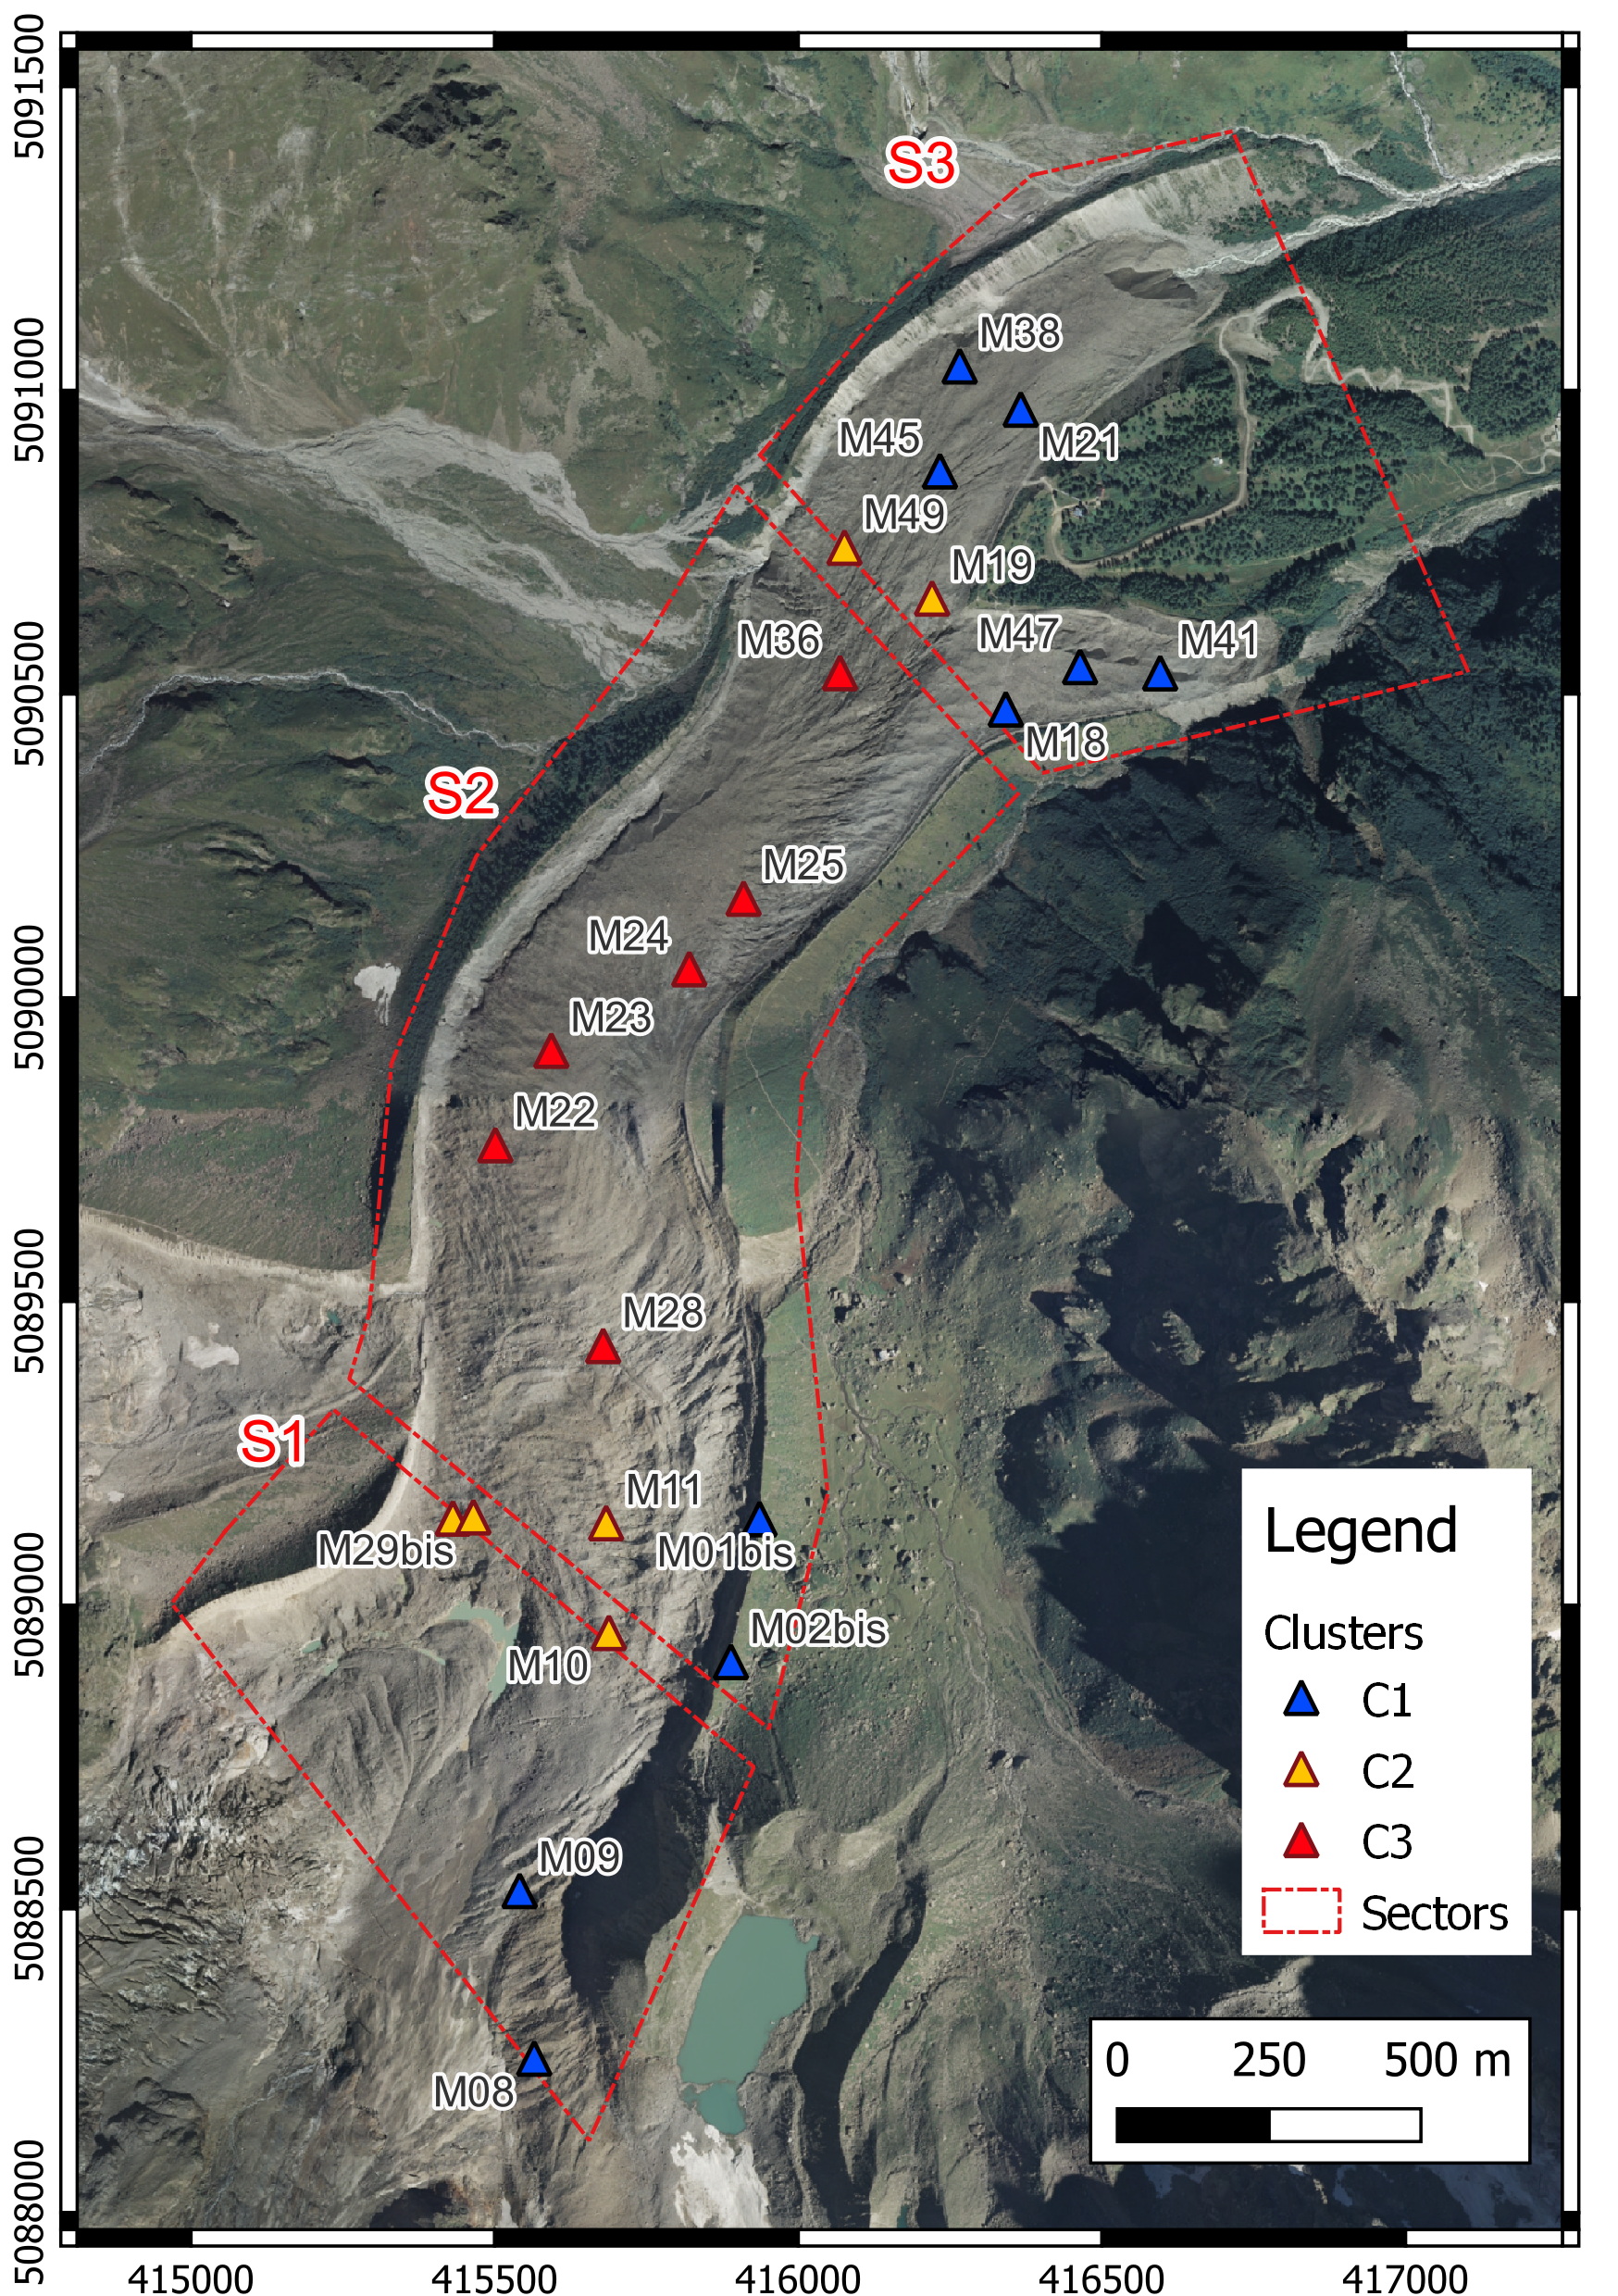
\includegraphics[width=0.29\textwidth]{GCPghiaccaio_clusters}
    }
    \caption{\textbf{(a)} Time series of the velocity computed from the GNSS measurements of the targets deployed over the glacier. Dashed lines denote measurement continuity over the years (i.e., if the line is interrupted, the target was lost or not measured during that year). Labels C1-C3 denote the three velocity clusters of GNSS points, whereas labels S1-S3 indicate the three morphological sectors marked in \figref{fig:belvedere}a. A correspondence between clusters and sectors can be identified: C1 corresponds to sectors S1 and S2, cluster C3 to sector S2, whereas cluster C2 corresponds to the two transition areas S2-S1 and S2-S3. \textbf{(b)} Location of the targets over the glacier. \textcolor{red}{UPDATE}}
    \label{fig:3:GNSS_velocity}		
\end{figure}

Annual ice flow velocities were first computed using in-situ GNSS measurements of moving targets
(\figref{fig:3:GNSS_velocity}).
Most of the moving targets were found and measured for 3 or more years and some of them have been continuously tracked since 2015 
(e.g.,\textit{M10}, \textit{M28}, \textit{M41}). 
While some targets were inevitably lost (e.g., due to presence of crevasses), they were replaced with new ones 
materialized nearby to maintain data continuity. 

Analysis of the graph in \figref{fig:3:GNSS_velocity} reveals three distinct velocity clusters (C1, C2, C3) 
within the GNSS data.  
Cluster C1 exhibits the lowest velocities \qtylist{2;7}{\meter\per\year} and encompasses points in the upper 
accumulation section and glacier tongues. 
Significantly faster speeds \qtylist{17;22}{\meter\per\year} characterize cluster C3, located in the glacier's 
central part (e.g., targets \textit{M10, M11, M22, M28}). 
Cluster C2 represents a transition zone with intermediate velocities, found between the central sector 
and the accumulation area (targets \textit{M10, M11}) and between the central sector and the lower north-west tongue 
(e.g., target \textit{M49}).

\begin{figure}[ht!]
    \centering
    \includegraphics[width=0.68\textwidth]{man_points_2015-2020}
    \caption{\textit{MAN} points between 2015-2020 \textcolor{red}{UPDATE. take only 2015-2017 (use 2018-2019 as valid for DIC}. Change colorscale to viridis}
    \label{fig:3:MAN_points_all}
\end{figure}

Additionally, orthophotos were used to derive a more complete flow velocity field.
Due to unfavorable conditions, from 2015 to 2017, it was not feasible to apply DIC to orthophotos
to automatically derive glacier displacement, but manually collimated points were used (\figref{fig:3:MAN_points_all}). 



\subsection{Volume variations \textcolor{red}{Update}}\label{sec:3:res:volumes}

\begin{figure}
    \centering
    \includegraphics[width=0.8\columnwidth]{volume_loss_2015-2023.png}
    \caption{Yearly volume variation computed as difference between DSM of two
        consecutive years. The~error bars plotted represent the uncertainty of each
        estimated value. Note that the values on the Y axis are expressed in million of
        \si{\cubic\meter}. \textcolor{red}{Update with 2021-2023}}
    \label{fig:3:volumes}
\end{figure}

\begin{figure}[ht!]
  \centering
  \subcaptionbox{\label{fig:3:profiles:AA}}{
    \includegraphics[width=.45\textwidth]{profile_AA.jpg}
  }
  \subcaptionbox{\label{fig:3:profiles:BB}}{
    \includegraphics[width=.45\textwidth]{profile_BB.jpg}
  }\\
  \subcaptionbox{\label{fig:3:profiles:CC}}{
    \includegraphics[width=.45\textwidth]{profile_CC.jpg}
  }
  \subcaptionbox{\label{fig:3:profiles:DD}}{
    \includegraphics[width=.45\textwidth]{profile_DD.jpg}
  } \\
  \subcaptionbox{\label{fig:3:profiles:map}}{
    \includegraphics[width=.45\textwidth]{profileMap.png}
  }
    \caption{Elevation profiles obtained from the DSM computed on the years 2015-2020 along 4 different cross-sections. \textbf{(a)} Cross-section AA' at the north-west glacier tongue; \textbf{(b)} Cross-section BB' at the south tongue; \textbf{(c)} Cross-section CC' in the lower portion of the glacier transition sector; \textbf{(d)} Cross-section DD' in the upper portion of the glacier transition sector; \textbf{(e)} Cross-sections location. Cross-sections are seen from South towards North (i.e., from upstream to downstream of the glacier), as marked by the letters in \textbf{(e)}. \textcolor{red}{ADD NEW PROFILES}}
    \label{fig:3:profiles}
\end{figure}

\figref{fig:3:volumes} illustrates the loss of ice volume year by year.
The estimated variance of the glacier volume variation is plotted as an error bar for
each value of volume~variation.

Between 2017 and 2018, field works were moved from Autumn to Summer.
Therefore, the~loss of volume for the year 2017--2018 was computed between October 2017
and July 2018, therefore it represented only the variation occurred in wintertime and
springtime, and~it should not be directly compared with the annual average.
Indeed, 2017--2018 volume variation was \SI{-0.75e6}{\cubic\meter}, against~the average
variation between 2015 and 2020 of \SI{-2.81e6}{\cubic\meter} (difference of
\SI{27}{\percent}).
Ice volume loss for the year 2019--2020 may be slightly underestimated as well: the
photogrammetric model of the upper part of the glacier was affected by a larger geometric
(RMSE in vertical direction of \SI{0.28}{\meter}, see \secref{sec:3:problems})
compared to the others models, due to the lack of GCPs measured in-situ at the time of
the photo acquisition.
Overall, the~negative ice volume variation occurred between 2015 and 2020 is evident and
significant: every year, between~\SIlist{2e6;3.5e6}{\cubic\meter} of ice were~lost.

In \figref{fig:3:profiles}, elevation profiles of the glacier obtained every year at four different cross sections are plotted together.
In each profile, it is easily identifiable the glacier surface, which is delimited by the lateral moraines.
The highest height reduction is found at the lower terminus of the glacier (\figref{fig:3:profiles}a-b): \qty{\sim 2}{\meter} have been lost every year. 
It is noticeable that the overall glacier surface profile remained the same, but the ice thickness shrank.
In the central part of the glacier (sections CC' and DD', \figref{fig:3:profiles}c-d), the height reduction was less regular because of the crevasses that strongly ripple the transfer zone of the glacier.	

% \subsection{Glacier outline \textcolor{red}{TODO}}\label{sec:3:res:outline}

% {\color{red} TODO}

\section{An open source database to store and share the monitoring results \textcolor{red}{TODO}}

{\color{red} TODO}

% \subsection{Morphological sectors\textcolor{red}{TODO}}\label{sec:3:discussion:sectors}

% \begin{figure}
%     \centering
%     \includegraphics[width=.7\textwidth]{belvedereMapSect}
% 	\caption{Subdivision of the Belvedere Glacier in three main morphological sectors: sector 1 (S1) is the accumulation zone, sector 2 (S2) is the transfer zone, sector 3 (S3) is the low-relief zone with the two glacier tongues. Coordinates are framed in ETRF2000(2008) UTM 32N. [Basemap source: \textit{Swisstopo (geo.admin.ch)}].}
% 	\label{fig:3:sectors}	
% \end{figure}	

% \subsection{Comparison with previous studies\textcolor{red}{UPDATE}}\label{sec:3:discussion:prevstudies}


\section{Comparison with previous studies}\label{sec:3:prevstudies}

Several studies focused on understanding and quantifying Belvedere Glacier
dynamics.~\cite{Kaab2005} estimated velocities ranging between
\SIlist{32;43}{\meter\per\year} on the whole Belvedere Glacier from October 1995 to
September 1999, by~employing aerial images.
Besides, velocities between \SIlist{100;200}{\meter\per\year} were estimated
by~\cite{Kaab2005} in Autumn 2001, during~the extraordinary surge event of 2000--2001.
Nowadays, the~Belvedere Glacier is clearly moving slower compared to the late 1990s.
However, to~the best of authors knowledge, there are no recent works estimating glacier
flow~velocities.

Concerning volume variations,~\cite{Diolaiuti2003} digitalized two large-scale
topographic maps to interpolate DSMs and estimate volume variations between 1957 and
1991.
They found a positive volume difference of
\SI[retain-explicit-plus]{+22.7e6}{\cubic\meter} (with an average rate of \SI{\sim
    0.69e6}{\cubic\m\per\year}, roughly assuming a linear volume variation during the
years).

Their result matched with the study of~\cite{Roethlisberger1985}, who estimated an
increase of the glacier height of \SI[retain-explicit-plus]{+1.5}{\m\per\year} between
1983 and 1985.
Recently,~\cite{Degaetani2021} used historical aerial images and UAVs to
photogrammetrically reconstruct glacier volume variations between 1977 and 2019.
For the period 1977--1991, they confirmed the glacier expansion, with~a volume
increase of \SI[retain-explicit-plus]{+10.06e6}{\cubic\meter}
(\SI[retain-explicit-plus]{+0.72e6}{\cubic\m\per\year}).
The expansion continued up to 2001 (at the end of the surge event), with~additional
\SI{10.61e6}{\cubic\m} of ice gained.
Since 2001, a~severe glacier retreat has begun, with~a loss of ice volume of
\SI{-47.78e6}{\cubic\meter} (\SI{-5.97e6}{\cubic\meter\per\year}) between 2001 and 2009.
For the time-span 2009--2019,~\citep{Degaetani2021} derived a negative variation of
\SI{-27.16e6}{\cubic\m} of ice (\SI{-2.72e6}{\cubic\meter\per\year}).
This last ten-years-averaged estimate well matches with the annual volume variations
found in this study between 2015 and 2020 (between
\SIlist{-2e6;-3.5e6}{\cubic\meter\per\year}).



% References
\makechapterbibliography{}

